% Created by tikzDevice version 0.12 on 2019-02-12 11:47:30
% !TEX encoding = UTF-8 Unicode
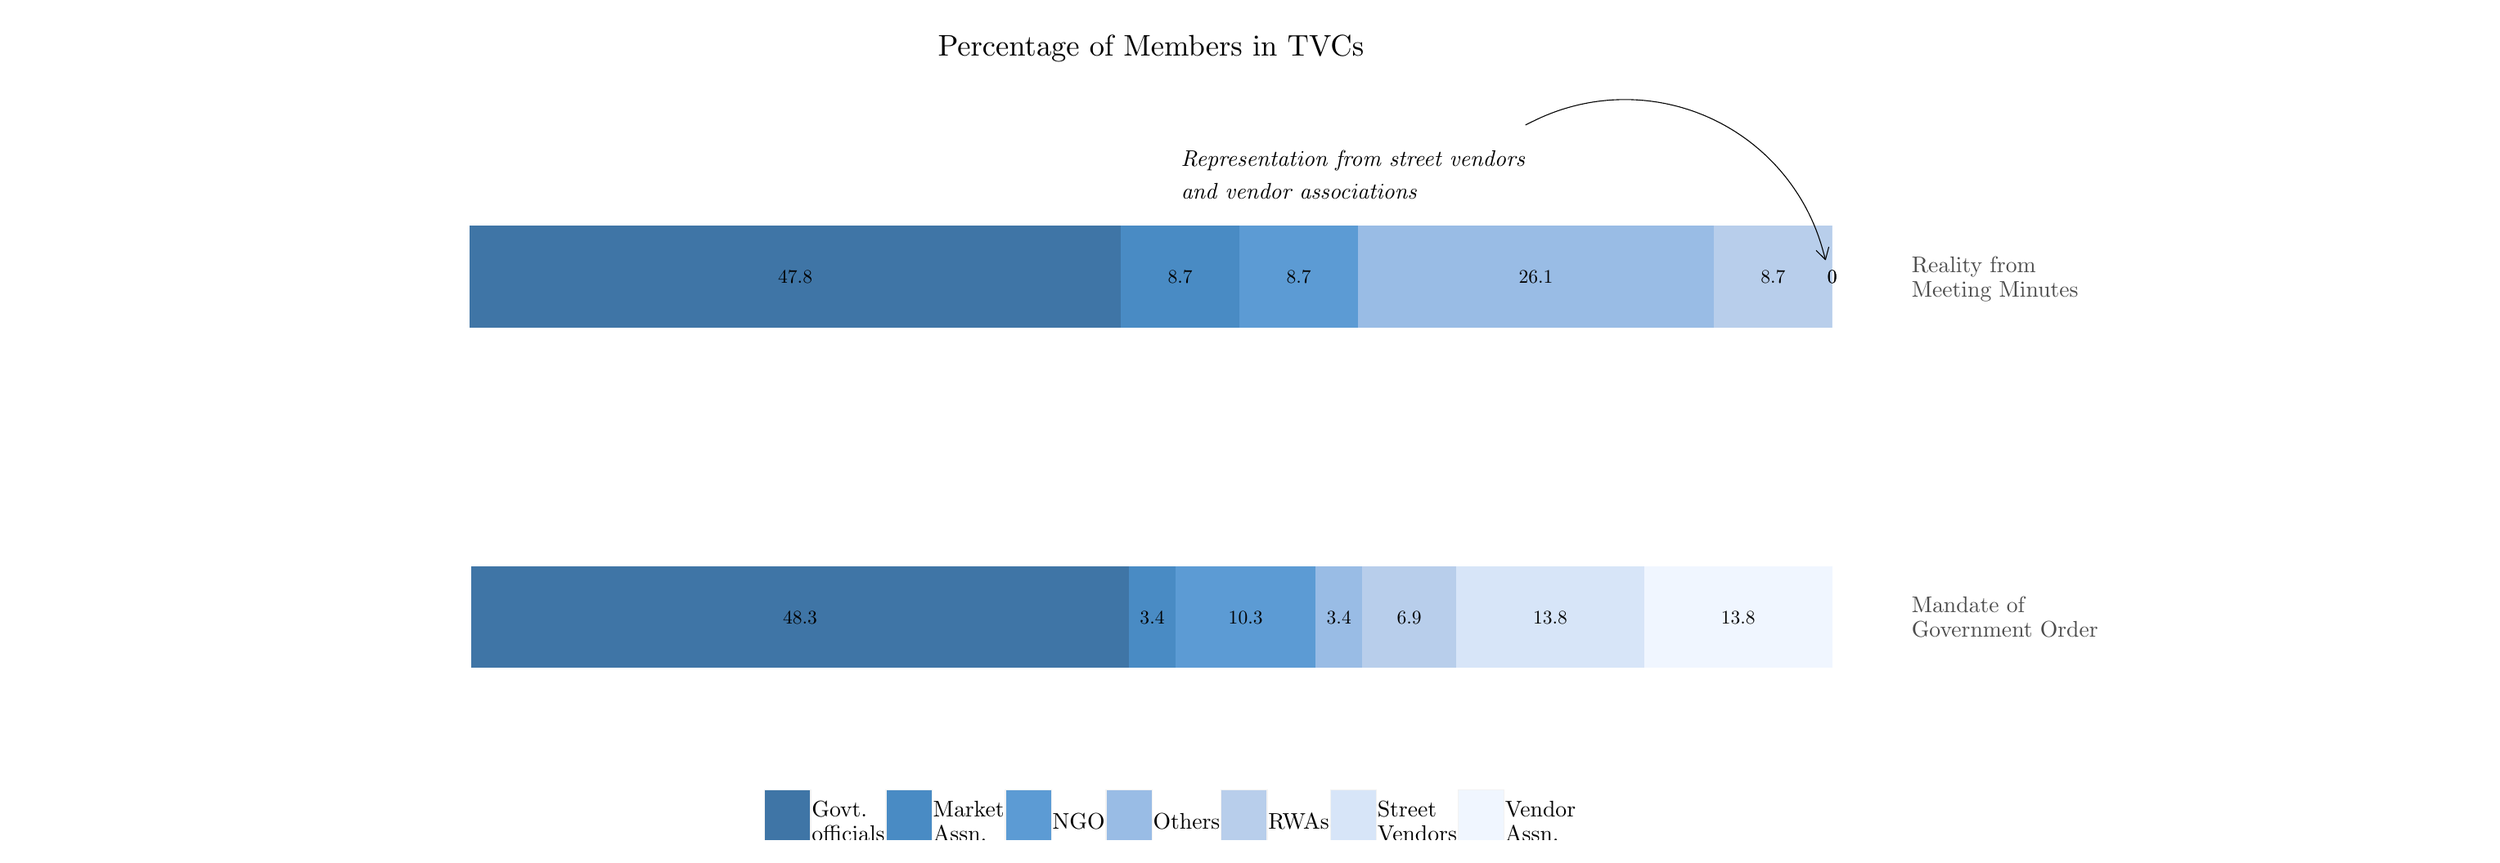
\begin{tikzpicture}[x=1pt,y=1pt]
\definecolor{fillColor}{RGB}{255,255,255}
\path[use as bounding box,fill=fillColor,fill opacity=0.00] (0,0) rectangle (1084.05,361.35);
\begin{scope}
\path[clip] (161.81,  0.00) rectangle (922.24,361.35);
\definecolor{drawColor}{RGB}{255,255,255}
\definecolor{fillColor}{RGB}{255,255,255}

\path[draw=drawColor,line width= 0.6pt,line join=round,line cap=round,fill=fillColor] (161.81,  0.00) rectangle (922.24,361.35);
\end{scope}
\begin{scope}
\path[clip] (167.31,  8.25) rectangle (829.44,339.31);
\definecolor{fillColor}{RGB}{240,246,255}

\path[fill=fillColor] (716.27, 75.97) rectangle (799.34,121.11);
\definecolor{fillColor}{RGB}{215,229,248}

\path[fill=fillColor] (633.21, 75.97) rectangle (716.27,121.11);
\definecolor{fillColor}{RGB}{184,206,235}

\path[fill=fillColor] (591.67, 75.97) rectangle (633.21,121.11);
\definecolor{fillColor}{RGB}{153,188,229}

\path[fill=fillColor] (571.21, 75.97) rectangle (591.67,121.11);
\definecolor{fillColor}{RGB}{92,155,212}

\path[fill=fillColor] (509.21, 75.97) rectangle (571.21,121.11);
\definecolor{fillColor}{RGB}{73,139,196}

\path[fill=fillColor] (488.74, 75.97) rectangle (509.21,121.11);
\definecolor{fillColor}{RGB}{63,117,166}

\path[fill=fillColor] (198.01, 75.97) rectangle (488.74,121.11);
\definecolor{fillColor}{RGB}{184,206,235}

\path[fill=fillColor] (746.97,226.45) rectangle (799.34,271.60);
\definecolor{fillColor}{RGB}{153,188,229}

\path[fill=fillColor] (589.87,226.45) rectangle (746.97,271.60);
\definecolor{fillColor}{RGB}{92,155,212}

\path[fill=fillColor] (537.50,226.45) rectangle (589.87,271.60);
\definecolor{fillColor}{RGB}{73,139,196}

\path[fill=fillColor] (485.13,226.45) rectangle (537.50,271.60);
\definecolor{fillColor}{RGB}{63,117,166}

\path[fill=fillColor] (197.40,226.45) rectangle (485.13,271.60);
\definecolor{fillColor}{RGB}{240,246,255}

\path[fill=fillColor] (799.34,226.45) rectangle (799.34,271.60);
\definecolor{fillColor}{RGB}{215,229,248}

\path[fill=fillColor] (799.34,226.45) rectangle (799.34,271.60);
\definecolor{drawColor}{RGB}{0,0,0}

\node[text=drawColor,anchor=base,inner sep=0pt, outer sep=0pt, scale=  0.85] at (757.81, 95.60) {13.8};

\node[text=drawColor,anchor=base,inner sep=0pt, outer sep=0pt, scale=  0.85] at (674.74, 95.60) {13.8};

\node[text=drawColor,anchor=base,inner sep=0pt, outer sep=0pt, scale=  0.85] at (612.44, 95.60) {6.9};

\node[text=drawColor,anchor=base,inner sep=0pt, outer sep=0pt, scale=  0.85] at (581.44, 95.60) {3.4};

\node[text=drawColor,anchor=base,inner sep=0pt, outer sep=0pt, scale=  0.85] at (540.21, 95.60) {10.3};

\node[text=drawColor,anchor=base,inner sep=0pt, outer sep=0pt, scale=  0.85] at (498.97, 95.60) {3.4};

\node[text=drawColor,anchor=base,inner sep=0pt, outer sep=0pt, scale=  0.85] at (343.37, 95.60) {48.3};

\node[text=drawColor,anchor=base,inner sep=0pt, outer sep=0pt, scale=  0.85] at (773.16,246.08) {8.7};

\node[text=drawColor,anchor=base,inner sep=0pt, outer sep=0pt, scale=  0.85] at (668.42,246.08) {26.1};

\node[text=drawColor,anchor=base,inner sep=0pt, outer sep=0pt, scale=  0.85] at (563.68,246.08) {8.7};

\node[text=drawColor,anchor=base,inner sep=0pt, outer sep=0pt, scale=  0.85] at (511.31,246.08) {8.7};

\node[text=drawColor,anchor=base,inner sep=0pt, outer sep=0pt, scale=  0.85] at (341.27,246.08) {47.8};

\node[text=drawColor,anchor=base,inner sep=0pt, outer sep=0pt, scale=  0.85] at (799.34,246.08) {0};

\node[text=drawColor,anchor=base,inner sep=0pt, outer sep=0pt, scale=  0.85] at (799.34,246.08) {0};

\path[draw=drawColor,line width= 0.4pt,line join=round,line cap=round] (663.90,316.14) --
	(664.16,316.27) --
	(665.42,316.88) --
	(667.26,317.78) --
	(668.91,318.57) --
	(670.23,319.19) --
	(671.13,319.59) --
	(672.32,320.11) --
	(673.62,320.64) --
	(674.99,321.19) --
	(676.37,321.71) --
	(677.66,322.18) --
	(678.59,322.50) --
	(679.82,322.91) --
	(681.15,323.33) --
	(682.57,323.75) --
	(683.99,324.15) --
	(685.31,324.50) --
	(686.27,324.74) --
	(687.53,325.04) --
	(688.90,325.34) --
	(690.35,325.63) --
	(691.79,325.91) --
	(693.15,326.14) --
	(694.12,326.29) --
	(695.40,326.48) --
	(696.79,326.66) --
	(698.26,326.82) --
	(699.73,326.97) --
	(701.09,327.08) --
	(702.08,327.15) --
	(703.37,327.22) --
	(704.77,327.27) --
	(706.25,327.31) --
	(707.72,327.33) --
	(709.09,327.32) --
	(710.08,327.30) --
	(711.37,327.25) --
	(712.77,327.19) --
	(714.25,327.09) --
	(715.72,326.98) --
	(717.08,326.85) --
	(718.06,326.74) --
	(719.35,326.58) --
	(720.73,326.39) --
	(722.20,326.17) --
	(723.65,325.92) --
	(725.00,325.67) --
	(725.96,325.48) --
	(727.23,325.21) --
	(728.60,324.90) --
	(730.04,324.55) --
	(731.46,324.18) --
	(732.78,323.81) --
	(733.72,323.53) --
	(734.96,323.15) --
	(736.30,322.72) --
	(737.70,322.24) --
	(739.08,321.75) --
	(740.37,321.26) --
	(741.28,320.90) --
	(742.49,320.42) --
	(743.77,319.87) --
	(745.13,319.27) --
	(746.46,318.65) --
	(747.70,318.06) --
	(748.58,317.62) --
	(749.73,317.03) --
	(750.97,316.37) --
	(752.27,315.65) --
	(753.54,314.92) --
	(754.72,314.22) --
	(755.56,313.71) --
	(756.66,313.01) --
	(757.83,312.25) --
	(759.06,311.42) --
	(760.26,310.58) --
	(761.38,309.78) --
	(762.17,309.19) --
	(763.20,308.40) --
	(764.30,307.54) --
	(765.45,306.60) --
	(766.57,305.66) --
	(767.61,304.76) --
	(768.35,304.11) --
	(769.31,303.24) --
	(770.33,302.28) --
	(771.39,301.25) --
	(772.43,300.21) --
	(773.38,299.22) --
	(774.06,298.51) --
	(774.94,297.55) --
	(775.87,296.50) --
	(776.84,295.38) --
	(777.78,294.26) --
	(778.64,293.19) --
	(779.25,292.42) --
	(780.04,291.39) --
	(780.88,290.26) --
	(781.74,289.06) --
	(782.58,287.86) --
	(783.35,286.72) --
	(783.89,285.90) --
	(784.59,284.80) --
	(785.32,283.61) --
	(786.08,282.33) --
	(786.81,281.06) --
	(787.47,279.86) --
	(787.94,278.99) --
	(788.53,277.84) --
	(789.16,276.59) --
	(789.80,275.25) --
	(790.41,273.92) --
	(790.97,272.66) --
	(791.35,271.75) --
	(791.85,270.55) --
	(792.36,269.25) --
	(792.88,267.86) --
	(793.37,266.48) --
	(793.82,265.18) --
	(794.12,264.25) --
	(794.51,263.00) --
	(794.94,261.53) --
	(795.46,259.68) --
	(796.00,257.76) --
	(796.29,256.68) --
	(796.33,256.55);

\path[draw=drawColor,line width= 0.4pt,line join=round,line cap=round] (792.28,260.55) --
	(796.33,256.55) --
	(797.77,262.05);
\end{scope}
\begin{scope}
\path[clip] (167.31,  8.25) rectangle (829.44,339.31);
\definecolor{drawColor}{RGB}{0,0,0}

\node[text=drawColor,anchor=base west,inner sep=0pt, outer sep=0pt, scale=  1.00] at (511.62,297.67) {\itshape Representation from street vendors};

\node[text=drawColor,anchor=base west,inner sep=0pt, outer sep=0pt, scale=  1.00] at (511.62,283.27) {\itshape and vendor associations};
\end{scope}
\begin{scope}
\path[clip] (  0.00,  0.00) rectangle (1084.05,361.35);
\definecolor{drawColor}{gray}{0.30}

\node[text=drawColor,anchor=base west,inner sep=0pt, outer sep=0pt, scale=  1.00] at (834.39,100.50) {Mandate of};

\node[text=drawColor,anchor=base west,inner sep=0pt, outer sep=0pt, scale=  1.00] at (834.39, 89.70) {Government Order};

\node[text=drawColor,anchor=base west,inner sep=0pt, outer sep=0pt, scale=  1.00] at (834.39,250.98) {Reality from};

\node[text=drawColor,anchor=base west,inner sep=0pt, outer sep=0pt, scale=  1.00] at (834.39,240.18) {Meeting Minutes};
\end{scope}
\begin{scope}
\path[clip] (  0.00,  0.00) rectangle (1084.05,361.35);
\definecolor{fillColor}{RGB}{255,255,255}

\path[fill=fillColor] (327.24, -5.98) rectangle (695.99, 22.48);
\end{scope}
\begin{scope}
\path[clip] (  0.00,  0.00) rectangle (1084.05,361.35);
\definecolor{drawColor}{RGB}{255,255,255}
\definecolor{fillColor}{gray}{0.95}

\path[draw=drawColor,line width= 0.6pt,line join=round,line cap=round,fill=fillColor] (327.24, -5.98) rectangle (348.58, 22.48);
\end{scope}
\begin{scope}
\path[clip] (  0.00,  0.00) rectangle (1084.05,361.35);
\definecolor{fillColor}{RGB}{63,117,166}

\path[fill=fillColor] (327.95, -5.27) rectangle (347.87, 21.77);
\end{scope}
\begin{scope}
\path[clip] (  0.00,  0.00) rectangle (1084.05,361.35);
\definecolor{drawColor}{RGB}{255,255,255}
\definecolor{fillColor}{gray}{0.95}

\path[draw=drawColor,line width= 0.6pt,line join=round,line cap=round,fill=fillColor] (380.85, -5.98) rectangle (402.19, 22.48);
\end{scope}
\begin{scope}
\path[clip] (  0.00,  0.00) rectangle (1084.05,361.35);
\definecolor{fillColor}{RGB}{73,139,196}

\path[fill=fillColor] (381.56, -5.27) rectangle (401.47, 21.77);
\end{scope}
\begin{scope}
\path[clip] (  0.00,  0.00) rectangle (1084.05,361.35);
\definecolor{drawColor}{RGB}{255,255,255}
\definecolor{fillColor}{gray}{0.95}

\path[draw=drawColor,line width= 0.6pt,line join=round,line cap=round,fill=fillColor] (433.59, -5.98) rectangle (454.93, 22.48);
\end{scope}
\begin{scope}
\path[clip] (  0.00,  0.00) rectangle (1084.05,361.35);
\definecolor{fillColor}{RGB}{92,155,212}

\path[fill=fillColor] (434.31, -5.27) rectangle (454.22, 21.77);
\end{scope}
\begin{scope}
\path[clip] (  0.00,  0.00) rectangle (1084.05,361.35);
\definecolor{drawColor}{RGB}{255,255,255}
\definecolor{fillColor}{gray}{0.95}

\path[draw=drawColor,line width= 0.6pt,line join=round,line cap=round,fill=fillColor] (478.05, -5.98) rectangle (499.39, 22.48);
\end{scope}
\begin{scope}
\path[clip] (  0.00,  0.00) rectangle (1084.05,361.35);
\definecolor{fillColor}{RGB}{153,188,229}

\path[fill=fillColor] (478.77, -5.27) rectangle (498.68, 21.77);
\end{scope}
\begin{scope}
\path[clip] (  0.00,  0.00) rectangle (1084.05,361.35);
\definecolor{drawColor}{RGB}{255,255,255}
\definecolor{fillColor}{gray}{0.95}

\path[draw=drawColor,line width= 0.6pt,line join=round,line cap=round,fill=fillColor] (528.91, -5.98) rectangle (550.25, 22.48);
\end{scope}
\begin{scope}
\path[clip] (  0.00,  0.00) rectangle (1084.05,361.35);
\definecolor{fillColor}{RGB}{184,206,235}

\path[fill=fillColor] (529.63, -5.27) rectangle (549.54, 21.77);
\end{scope}
\begin{scope}
\path[clip] (  0.00,  0.00) rectangle (1084.05,361.35);
\definecolor{drawColor}{RGB}{255,255,255}
\definecolor{fillColor}{gray}{0.95}

\path[draw=drawColor,line width= 0.6pt,line join=round,line cap=round,fill=fillColor] (577.11, -5.98) rectangle (598.45, 22.48);
\end{scope}
\begin{scope}
\path[clip] (  0.00,  0.00) rectangle (1084.05,361.35);
\definecolor{fillColor}{RGB}{215,229,248}

\path[fill=fillColor] (577.82, -5.27) rectangle (597.74, 21.77);
\end{scope}
\begin{scope}
\path[clip] (  0.00,  0.00) rectangle (1084.05,361.35);
\definecolor{drawColor}{RGB}{255,255,255}
\definecolor{fillColor}{gray}{0.95}

\path[draw=drawColor,line width= 0.6pt,line join=round,line cap=round,fill=fillColor] (633.52, -5.98) rectangle (654.86, 22.48);
\end{scope}
\begin{scope}
\path[clip] (  0.00,  0.00) rectangle (1084.05,361.35);
\definecolor{fillColor}{RGB}{240,246,255}

\path[fill=fillColor] (634.23, -5.27) rectangle (654.15, 21.77);
\end{scope}
\begin{scope}
\path[clip] (  0.00,  0.00) rectangle (1084.05,361.35);
\definecolor{drawColor}{RGB}{0,0,0}

\node[text=drawColor,anchor=base west,inner sep=0pt, outer sep=0pt, scale=  1.00] at (348.58, 10.21) {Govt.};

\node[text=drawColor,anchor=base west,inner sep=0pt, outer sep=0pt, scale=  1.00] at (348.58, -0.59) {officials};
\end{scope}
\begin{scope}
\path[clip] (  0.00,  0.00) rectangle (1084.05,361.35);
\definecolor{drawColor}{RGB}{0,0,0}

\node[text=drawColor,anchor=base west,inner sep=0pt, outer sep=0pt, scale=  1.00] at (402.19, 10.21) {Market};

\node[text=drawColor,anchor=base west,inner sep=0pt, outer sep=0pt, scale=  1.00] at (402.19, -0.59) {Assn.};
\end{scope}
\begin{scope}
\path[clip] (  0.00,  0.00) rectangle (1084.05,361.35);
\definecolor{drawColor}{RGB}{0,0,0}

\node[text=drawColor,anchor=base west,inner sep=0pt, outer sep=0pt, scale=  1.00] at (454.93,  4.81) {NGO};
\end{scope}
\begin{scope}
\path[clip] (  0.00,  0.00) rectangle (1084.05,361.35);
\definecolor{drawColor}{RGB}{0,0,0}

\node[text=drawColor,anchor=base west,inner sep=0pt, outer sep=0pt, scale=  1.00] at (499.39,  4.81) {Others};
\end{scope}
\begin{scope}
\path[clip] (  0.00,  0.00) rectangle (1084.05,361.35);
\definecolor{drawColor}{RGB}{0,0,0}

\node[text=drawColor,anchor=base west,inner sep=0pt, outer sep=0pt, scale=  1.00] at (550.25,  4.81) {RWAs};
\end{scope}
\begin{scope}
\path[clip] (  0.00,  0.00) rectangle (1084.05,361.35);
\definecolor{drawColor}{RGB}{0,0,0}

\node[text=drawColor,anchor=base west,inner sep=0pt, outer sep=0pt, scale=  1.00] at (598.45, 10.21) {Street};

\node[text=drawColor,anchor=base west,inner sep=0pt, outer sep=0pt, scale=  1.00] at (598.45, -0.59) {Vendors};
\end{scope}
\begin{scope}
\path[clip] (  0.00,  0.00) rectangle (1084.05,361.35);
\definecolor{drawColor}{RGB}{0,0,0}

\node[text=drawColor,anchor=base west,inner sep=0pt, outer sep=0pt, scale=  1.00] at (654.86, 10.21) {Vendor};

\node[text=drawColor,anchor=base west,inner sep=0pt, outer sep=0pt, scale=  1.00] at (654.86, -0.59) {Assn.};
\end{scope}
\begin{scope}
\path[clip] (  0.00,  0.00) rectangle (1084.05,361.35);
\definecolor{drawColor}{RGB}{0,0,0}

\node[text=drawColor,anchor=base,inner sep=0pt, outer sep=0pt, scale=  1.32] at (498.37,346.76) {Percentage of Members in TVCs};
\end{scope}
\end{tikzpicture}
